\documentclass[11pt,a4paper]{article}
\usepackage[margin=2.3cm]{geometry}
\usepackage{amsmath,amssymb}
\usepackage{siunitx}
\usepackage{tikz}
\usetikzlibrary{arrows.meta,calc}
\usepackage{pgfplots}
\pgfplotsset{compat=1.18}
\usepackage{booktabs}
\usepackage{xcolor}
\usepackage[hidelinks]{hyperref}

\definecolor{panel}{HTML}{1F4E79}
\definecolor{normal}{HTML}{C0392B}
\definecolor{vert}{HTML}{1E8449}
\definecolor{lat}{HTML}{D68910}

\newcommand{\vect}[1]{\mathbf{#1}}
\tikzset{
  vec/.style={-{Stealth[length=2.6mm]}, line width=0.9pt},
  axis/.style={-{Latex[length=2.2mm]}, line width=0.6pt, gray!70!black},
  pan/.style={line width=2.4pt, panel, line cap=round},
  dimn/.style={dashed, gray},
}

\title{The V-tail equivalence\\[2pt]
\large $S_{h,\mathrm{eff}} = \sum_i S_i\cos^2\nu_i$ and $S_{v,\mathrm{eff}} = \sum_i S_i\sin^2\nu_i$ in linear theory}
\author{da3Dalus calculation canon --- derivation note for GH \#1208}
\date{28 October 2026}

\begin{document}
\maketitle

\begin{abstract}
A V-tail panel of true (developed) area $S$ and lift-curve slope $a$, inclined by the dihedral
angle $\nu$, contributes $a S\cos^2\nu$ to the pitch-force derivative and $a S\sin^2\nu$ to the
side-force derivative. One factor $\cos\nu$ (or $\sin\nu$) comes from projecting the free-stream
incidence onto the panel normal, the other from projecting the panel's normal force back onto the
body axes. This note derives the result step by step, generalises it to polyhedral tails, lists the
limit checks, and separates what is exact in linear theory from what is an assumption.
\end{abstract}

\section{Step 1 --- Axes and geometry}

\paragraph{Assumptions.} Rigid aircraft; body axes with $x$ forward, $y$ to the right
(starboard), $z$ \emph{up}. (Standard flight-mechanics body axes have $z$ down; that only flips the
sign of the vertical force $Z$.) The tail is mirror-symmetric about the $x$--$z$ plane. Each panel is
flat, with true area $S$ (measured in its own plane) and dihedral angle $\nu$ to the horizontal.

\paragraph{Geometry.} The spanwise unit vectors $\vect{s}$ and the panel normals $\vect{n}$ (in
$(x,y,z)$ components) are
\begin{align}
  \vect{s}_R &= (0,\ \cos\nu,\ \sin\nu), &
  \vect{n}_R &= (0,\ -\sin\nu,\ \cos\nu), \label{eq:nR}\\
  \vect{s}_L &= (0,\ -\cos\nu,\ \sin\nu), &
  \vect{n}_L &= (0,\ +\sin\nu,\ \cos\nu). \label{eq:nL}
\end{align}
$\vect{n}_R$ is the vertical unit vector $\vect{e}_z$ rotated by $+\nu$ about $x$; $\vect{n}_L$ is
$\vect{e}_z$ rotated by $-\nu$. Both normals point ``up and inboard'' (Fig.~\ref{fig:rear}).

\begin{figure}[ht]
\centering
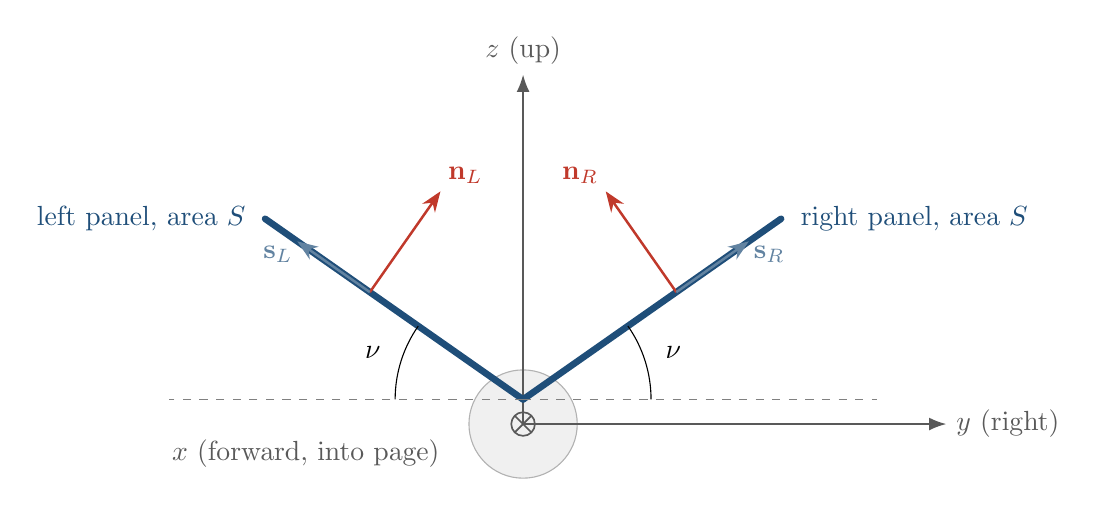
\begin{tikzpicture}[scale=1.25]
  \def\NU{35}
  \def\L{3.2}
  % fuselage
  \draw[fill=gray!12, draw=gray!60] (0,-0.25) circle (0.55);
  % axes
  \draw[axis] (0,-0.25) -- (4.3,-0.25) node[right] {$y$ (right)};
  \draw[axis] (0,-0.25) -- (0,3.3) node[above] {$z$ (up)};
  \draw[gray!70!black, line width=0.6pt] (0,-0.25) circle (0.12);
  \draw[gray!70!black, line width=0.6pt] (-0.085,-0.335) -- (0.085,-0.165) (-0.085,-0.165) -- (0.085,-0.335);
  \node[gray!70!black, anchor=east] at (-0.75,-0.55) {$x$ (forward, into page)};
  % panels
  \draw[pan] (0,0) -- (\NU:\L) coordinate (TR);
  \draw[pan] (0,0) -- (180-\NU:\L) coordinate (TL);
  \node[panel, anchor=west] at ($(TR)+(0.1,0)$) {right panel, area $S$};
  \node[panel, anchor=east] at ($(TL)+(-0.1,0)$) {left panel, area $S$};
  % horizontal reference + nu arcs
  \draw[dimn] (0,0) -- (3.6,0);
  \draw[dimn] (0,0) -- (-3.6,0);
  \draw[thin] (1.3,0) arc (0:\NU:1.3);
  \node at ({\NU/2}:1.6) {$\nu$};
  \draw[thin] (-1.3,0) arc (180:180-\NU:1.3);
  \node at ({180-\NU/2}:1.6) {$\nu$};
  % normals at mid-panel
  \coordinate (MR) at (\NU:{\L/2+0.3});
  \coordinate (ML) at (180-\NU:{\L/2+0.3});
  \draw[vec, normal] (MR) -- ++({90+\NU}:1.25) node[above left=-1pt] {$\vect{n}_R$};
  \draw[vec, normal] (ML) -- ++({90-\NU}:1.25) node[above right=-1pt] {$\vect{n}_L$};
  \draw[vec, panel!70] (MR) -- ++(\NU:0.9) node[below right=-2pt] {$\vect{s}_R$};
  \draw[vec, panel!70] (ML) -- ++(180-\NU:0.9) node[below left=-2pt] {$\vect{s}_L$};
\end{tikzpicture}
\caption{Rear view (looking forward). Each panel lies at dihedral $\nu$ to the horizontal; its
normal $\vect{n}$ is the vertical axis rotated by $\pm\nu$ about $x$. Drawn for $\nu=\ang{35}$.}
\label{fig:rear}
\end{figure}

\section{Step 2 --- Incidence normal to the panel}

\paragraph{Assumptions.} Small angle of attack $\alpha$ and small sideslip $\beta$ (with $\beta>0$
meaning wind from starboard); $\alpha$ and $\beta$ are the \emph{local} values at the tail, i.e.\ they
already contain downwash and sidewash. First order in $\alpha,\beta$ throughout.

\paragraph{Equation.} The air velocity relative to the aircraft is
\begin{equation}
  \vect{V}_\mathrm{air} = V\,(-\cos\alpha\cos\beta,\ -\sin\beta,\ \sin\alpha)
  \approx V\,(-1,\ -\beta,\ \alpha). \label{eq:vair}
\end{equation}
The chordwise component is $V$ to first order, so the panel's normal incidence is
$\alpha_n = \vect{V}_\mathrm{air}\cdot\vect{n}/V$. With \eqref{eq:nR}--\eqref{eq:nL}:
\begin{equation}
  \boxed{\alpha_{n,R} = \alpha\cos\nu + \beta\sin\nu,\qquad
         \alpha_{n,L} = \alpha\cos\nu - \beta\sin\nu.} \label{eq:alphan}
\end{equation}

\paragraph{In words.} An upward crossflow $V\alpha$ meets a tilted panel; only its component along
the normal, $V\alpha\cos\nu$, is an incidence. A crossflow from starboard, $V\beta$, has the component
$V\beta\sin\nu$ along the normals, with opposite sign on the two panels: it pushes the
right panel on its outer (lower) face and the left panel on its inner (upper) face (Fig.~\ref{fig:incidence}).

\begin{figure}[ht]
\centering
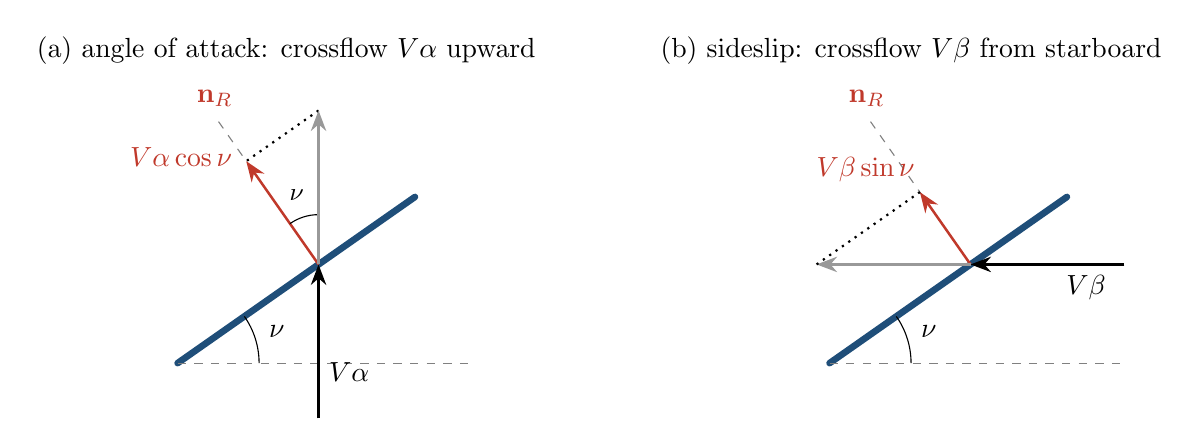
\begin{tikzpicture}[scale=1.15]
  \def\NU{35}
  % ---------- (a) alpha ----------
  \begin{scope}
    \node at (1.2,3.45) {(a) angle of attack: crossflow $V\alpha$ upward};
    \draw[pan] (0,0) -- (\NU:3.2);
    \draw[dimn] (0,0) -- (3.3,0);
    \draw[thin] (0.9,0) arc (0:\NU:0.9); \node at ({\NU/2}:1.15) {$\nu$};
    \coordinate (P) at (\NU:1.9);
    \draw[vec, black] ($(P)+(0,-1.7)$) -- (P) node[pos=0.3, right] {$V\alpha$};
    % normal direction and projection
    \draw[dimn] (P) -- ++({90+\NU}:2.0) coordinate (Ntip);
    \node[normal, anchor=south] at (Ntip) {$\vect{n}_R$};
    \draw[vec, normal] (P) -- ++({90+\NU}:1.392) coordinate (Q);
    \node[normal, anchor=east] at ($(Q)+(-0.05,0.05)$) {$V\alpha\cos\nu$};
    \draw[thin] (P) ++(0,0.55) arc (90:{90+\NU}:0.55);
    \node at ($(P)+({90+\NU/2}:0.8)$) {\small$\nu$};
    \draw[dotted, thick] ($(P)+(0,1.7)$) -- (Q);
    \draw[vec, black!40] (P) -- ++(0,1.7);
  \end{scope}
  % ---------- (b) beta ----------
  \begin{scope}[xshift=7.2cm]
    \node at (0.9,3.45) {(b) sideslip: crossflow $V\beta$ from starboard};
    \draw[pan] (0,0) -- (\NU:3.2);
    \draw[dimn] (0,0) -- (3.3,0);
    \draw[thin] (0.9,0) arc (0:\NU:0.9); \node at ({\NU/2}:1.15) {$\nu$};
    \coordinate (P) at (\NU:1.9);
    \draw[vec, black] ($(P)+(1.7,0)$) -- (P) node[pos=0.25, below] {$V\beta$};
    \draw[dimn] (P) -- ++({90+\NU}:2.0) coordinate (Ntip);
    \node[normal, anchor=south] at (Ntip) {$\vect{n}_R$};
    \draw[vec, normal] (P) -- ++({90+\NU}:0.975) coordinate (Q);
    \node[normal, anchor=south east] at ($(Q)+(0.05,0.0)$) {$V\beta\sin\nu$};
    \draw[vec, black!40] (P) -- ++(-1.7,0);
    \draw[dotted, thick] ($(P)+(-1.7,0)$) -- (Q);
  \end{scope}
\end{tikzpicture}
\caption{Projection of the crossflow onto the normal of the right panel (rear view). Grey
arrow: crossflow vector moved to the panel; red: its component along $\vect{n}_R$. (a)
$\alpha_n=\alpha\cos\nu$; (b) $\alpha_n=+\beta\sin\nu$ on the right panel, $-\beta\sin\nu$ on the
left (mirror image, not drawn).}
\label{fig:incidence}
\end{figure}

\section{Step 3 --- Normal force and its projection}

\paragraph{Assumptions.} Linear, attached flow. The panel force is normal to the panel:
by Kutta--Joukowski $\vect{F}=\rho\,\vect{V}\times\vect{\Gamma}$ with $\vect{V}\parallel x$ and
$\vect{\Gamma}\parallel\vect{s}$, so $\vect{F}\parallel\vect{n}$. The normal-force slope of the panel
is $a$ (per radian, based on the true area $S$); see Step~4 for which $a$.

\paragraph{Equation.}
\begin{equation}
  \vect{F}_i = q\,S\,a\,\alpha_{n,i}\,\vect{n}_i ,\qquad q=\tfrac12\rho V^2,\quad i\in\{R,L\}.
  \label{eq:force}
\end{equation}
Projecting onto $z$ and $y$ with \eqref{eq:nR}--\eqref{eq:nL} and inserting \eqref{eq:alphan}:
\begin{align}
  Z &= qSa\cos\nu\,(\alpha_{n,R}+\alpha_{n,L}) = 2qSa\,\alpha\cos^2\nu, \label{eq:Z}\\
  Y &= qSa\sin\nu\,(\alpha_{n,L}-\alpha_{n,R}) = -2qSa\,\beta\sin^2\nu. \label{eq:Y}
\end{align}
With $S_\mathrm{tot}=2S$:
\begin{equation}
  \boxed{\frac{\partial Z}{\partial\alpha} = q\,a\,S_\mathrm{tot}\cos^2\nu,\qquad
         \frac{\partial Y}{\partial\beta} = -q\,a\,S_\mathrm{tot}\sin^2\nu.} \label{eq:result}
\end{equation}

\paragraph{In words.} The first $\cos\nu$ is the incidence projection \eqref{eq:alphan}; the second
is the projection of the normal force onto the vertical (Fig.~\ref{fig:force}). The same holds with
$\sin\nu$ for sideslip. The cross terms cancel for the mirror pair: in the $\alpha$ case the lateral
components $\mp N\sin\nu$ of the two panels are equal and opposite; in the $\beta$ case the vertical
components are. A \emph{single} panel does couple, $\partial Z/\partial\beta = \pm qSa\sin\nu\cos\nu$.
The sign in \eqref{eq:result} is the usual fin sign: wind from starboard pushes the tail to port.

\begin{figure}[ht]
\centering
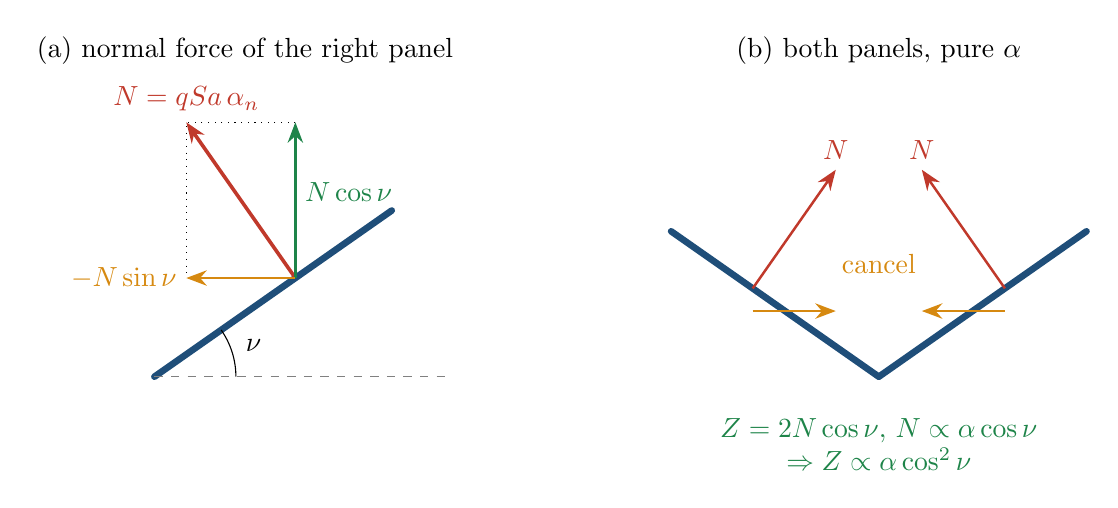
\begin{tikzpicture}[scale=1.15]
  \def\NU{35}
  % (a) single panel decomposition
  \begin{scope}
    \node at (1.0,3.6) {(a) normal force of the right panel};
    \draw[pan] (0,0) -- (\NU:3.2);
    \draw[dimn] (0,0) -- (3.3,0);
    \draw[thin] (0.9,0) arc (0:\NU:0.9); \node at ({\NU/2}:1.15) {$\nu$};
    \coordinate (P) at (\NU:1.9);
    \draw[vec, normal, line width=1.3pt] (P) -- ++({90+\NU}:2.1) coordinate (N)
        node[above] {$N = qSa\,\alpha_n$};
    \draw[vec, vert] (P) -- ($(P)+(0,{2.1*cos(\NU)})$) coordinate (V);
    \draw[vec, lat] (P) -- ($(P)+({-2.1*sin(\NU)},0)$) coordinate (H);
    \node[vert, anchor=west] at ($(P)!0.55!(V)$) {$N\cos\nu$};
    \node[lat, anchor=east] at (H) {$-N\sin\nu$};
    \draw[dotted] (V) -- (N) -- (H);
  \end{scope}
  % (b) pair in pitch
  \begin{scope}[xshift=8.0cm]
    \node at (0,3.6) {(b) both panels, pure $\alpha$};
    \draw[pan] (0,0) -- (\NU:2.8);
    \draw[pan] (0,0) -- (180-\NU:2.8);
    \coordinate (PR) at (\NU:1.7);
    \coordinate (PL) at (180-\NU:1.7);
    \draw[vec, normal] (PR) -- ++({90+\NU}:1.6) node[above] {$N$};
    \draw[vec, normal] (PL) -- ++({90-\NU}:1.6) node[above] {$N$};
    \draw[vec, lat] ($(PR)+(0,-0.25)$) -- ++({-1.6*sin(\NU)},0);
    \draw[vec, lat] ($(PL)+(0,-0.25)$) -- ++({1.6*sin(\NU)},0);
    \node[lat] at (0,1.25) {cancel};
    \node[vert, align=center] at (0,-0.75) {$Z = 2N\cos\nu$, $N\propto\alpha\cos\nu$\\
      $\Rightarrow Z\propto\alpha\cos^2\nu$};
  \end{scope}
\end{tikzpicture}
\caption{(a) The normal force $N$ splits into a vertical part $N\cos\nu$ and a lateral part
$N\sin\nu$. (b) For pure $\alpha$ both panels carry the same $N\propto\alpha\cos\nu$; the lateral
parts cancel, the vertical parts add to $Z\propto\alpha\cos^2\nu$. For pure $\beta$ the panels carry
opposite $N\propto\pm\beta\sin\nu$; the vertical parts cancel and the lateral parts add to
$Y\propto-\beta\sin^2\nu$.}
\label{fig:force}
\end{figure}

\section{Step 4 --- Which lift-curve slope, and why a single \texorpdfstring{$\cos\nu$}{cos nu} is wrong}

\paragraph{Which $a$.} The panel builds its circulation in its own plane, so $a$ belongs to the
\emph{true, developed} planform --- not to its shadow on the horizontal or vertical plane. For the
limit $\nu\to0$ to reproduce a flat tail, the aspect ratio must be that of the flattened pair:
\begin{equation}
  A = \frac{(2l)^2}{S_\mathrm{tot}} = \frac{2l^2}{S}, \label{eq:AR}
\end{equation}
with $l$ the panel length along its span (root to tip), not the semi-span value $l^2/S$.

\paragraph{Rotation invariance.} The response of the panel set to a crossflow
$\vect{w} = V(0,-\beta,\alpha)$ is linear, $\vect{F} = \mathsf{K}\,\vect{w}/V$, with
\begin{equation}
  \mathsf{K} = q\,a\sum_i S_i\,\vect{n}_i\vect{n}_i^{\mathsf{T}},\qquad
  K_{zz} = qa\sum_i S_i\cos^2\nu_i,\quad K_{yy} = qa\sum_i S_i\sin^2\nu_i. \label{eq:K}
\end{equation}
$\vect{n}\vect{n}^{\mathsf T}$ does not depend on which way $\vect{n}$ points. Rotating the whole
tail about $x$ only rotates $\mathsf K$, so its trace $K_{yy}+K_{zz}=qa\sum_i S_i$ cannot change.
This is the identity $\cos^2\nu+\sin^2\nu=1$.

\paragraph{The rejected variants.}
\begin{itemize}
  \item \emph{Projected area} $S\cos\nu$ with $a(A)$ drops the incidence projection. At
        $\nu=\ang{45}$ it gives $S_h+S_v=\sqrt2\,S_\mathrm{tot}$: a tilted flat surface would gain
        41\,\% effectiveness from nothing, violating the trace invariance.
  \item \emph{Projected aspect ratio} $(l\cos\nu)^2/(S\cos\nu)=A\cos\nu$ describes the shadow,
        which carries no circulation.
\end{itemize}
Fig.~\ref{fig:plot} compares the two laws.

\begin{figure}[ht]
\centering
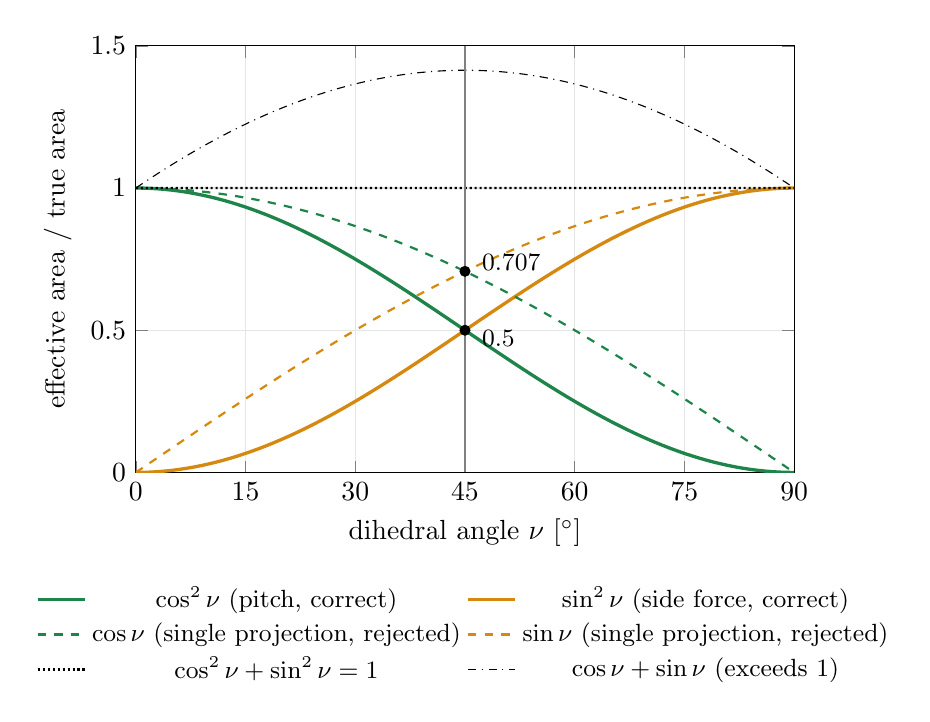
\begin{tikzpicture}
\begin{axis}[
  width=0.82\textwidth, height=7cm,
  xmin=0, xmax=90, ymin=0, ymax=1.5,
  xtick={0,15,30,45,60,75,90},
  xlabel={dihedral angle $\nu$ [\si{\degree}]},
  ylabel={effective area / true area},
  legend style={at={(0.5,-0.24)}, anchor=north, legend columns=2, font=\small, draw=none},
  grid=major, grid style={gray!20},
  samples=91, domain=0:90,
]
  \addplot[vert, very thick] {cos(x)^2};
  \addlegendentry{$\cos^2\nu$ (pitch, correct)}
  \addplot[lat, very thick] {sin(x)^2};
  \addlegendentry{$\sin^2\nu$ (side force, correct)}
  \addplot[vert, thick, dashed] {cos(x)};
  \addlegendentry{$\cos\nu$ (single projection, rejected)}
  \addplot[lat, thick, dashed] {sin(x)};
  \addlegendentry{$\sin\nu$ (single projection, rejected)}
  \addplot[black, densely dotted, thick] {cos(x)^2+sin(x)^2};
  \addlegendentry{$\cos^2\nu+\sin^2\nu = 1$}
  \addplot[black, dash dot] {cos(x)+sin(x)-0.0001};
  \addlegendentry{$\cos\nu+\sin\nu$ (exceeds 1)}
  \draw[gray] (axis cs:45,0) -- (axis cs:45,1.5);
  \fill (axis cs:45,0.5) circle (2pt);
  \fill (axis cs:45,0.7071) circle (2pt);
  \node[anchor=west, font=\small] at (axis cs:46,0.47) {$0.5$};
  \node[anchor=west, font=\small] at (axis cs:46,0.74) {$0.707$};
\end{axis}
\end{tikzpicture}
\caption{Effective-area factors over $\nu$. The correct laws cross at $\nu=\ang{45}$ with $0.5$ each
and always sum to $1$. The single-projection variant gives $0.707$ each at \ang{45}, and its sum
reaches $\sqrt2$.}
\label{fig:plot}
\end{figure}

\section{Step 5 --- Polyhedral tails: summing segments}

\paragraph{Assumptions.} (a) Small angles and attached flow, so each segment's force is linear in its
own $\alpha_{n,i}$. (b) The same normal-force slope per unit area on every segment; strictly the weight
is the local load, and tip segments carry less than their area share. (c) Mutual induction between
segments and between tail and fuselage is fully absorbed into the common $a$.

\paragraph{Equation.} By linearity, \eqref{eq:K} holds for any set of flat segments, giving
\begin{equation}
  \boxed{S_{h,\mathrm{eff}} = \sum_i S_i\cos^2\nu_i,\qquad S_{v,\mathrm{eff}} = \sum_i S_i\sin^2\nu_i,}
  \qquad S_{h,\mathrm{eff}}+S_{v,\mathrm{eff}} = \sum_i S_i . \label{eq:sum}
\end{equation}
The off-diagonal term is $K_{yz} = -qa\sum_i S_i\sin\nu_i\cos\nu_i$ with $\nu_i$ signed ($+$ right,
$-$ left). It vanishes for a mirror-symmetric layout. For a layout that is not mirror-symmetric
(single panel, inverted Y, an unmirrored kink) it does not vanish: $\alpha$ then produces side force
and $\beta$ produces lift, and that coupling must be carried rather than dropped.

\begin{figure}[ht]
\centering
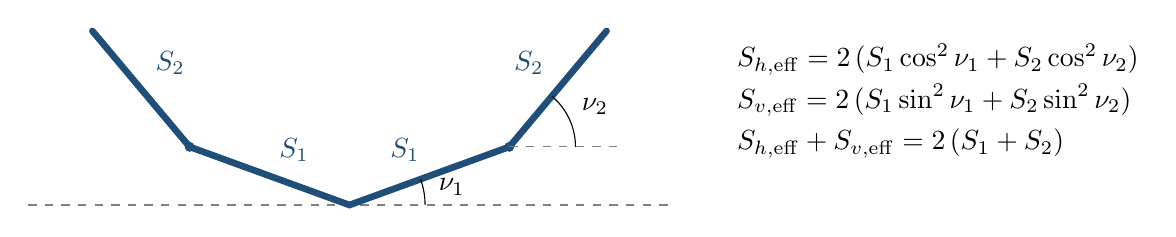
\begin{tikzpicture}[scale=1.2]
  \def\nua{20} \def\nub{50}
  \def\la{1.8} \def\lb{1.6}
  \coordinate (O) at (0,0);
  \coordinate (KR) at (\nua:\la);
  \coordinate (TR) at ($(KR)+(\nub:\lb)$);
  \coordinate (KL) at (180-\nua:\la);
  \coordinate (TL) at ($(KL)+(180-\nub:\lb)$);
  \draw[dimn] (-3.4,0) -- (3.4,0);
  \draw[pan] (TL) -- (KL) -- (O) -- (KR) -- (TR);
  \fill[panel] (KR) circle (1.5pt) (KL) circle (1.5pt);
  \draw[thin] (0.8,0) arc (0:\nua:0.8); \node at ({\nua/2}:1.1) {$\nu_1$};
  \draw[dimn] (KR) -- ++(1.2,0);
  \draw[thin] ($(KR)+(0.7,0)$) arc (0:\nub:0.7); \node at ($(KR)+({\nub/2}:1.0)$) {$\nu_2$};
  \node[panel, anchor=south east] at ($(O)!0.5!(KR)+(0,0.05)$) {$S_1$};
  \node[panel, anchor=south east] at ($(KR)!0.5!(TR)+(-0.05,0.05)$) {$S_2$};
  \node[panel, anchor=south west] at ($(O)!0.5!(KL)+(0,0.05)$) {$S_1$};
  \node[panel, anchor=south west] at ($(KL)!0.5!(TL)+(0.05,0.05)$) {$S_2$};
  \node[anchor=west, align=left] at (4.0,1.1) {%
    $S_{h,\mathrm{eff}} = 2\,(S_1\cos^2\nu_1 + S_2\cos^2\nu_2)$\\[3pt]
    $S_{v,\mathrm{eff}} = 2\,(S_1\sin^2\nu_1 + S_2\sin^2\nu_2)$\\[3pt]
    $S_{h,\mathrm{eff}}+S_{v,\mathrm{eff}} = 2\,(S_1+S_2)$};
\end{tikzpicture}
\caption{Polyhedral V-tail with an inner segment at $\nu_1$ and an outer segment at $\nu_2$ per
side (rear view, $\nu_1=\ang{20}$, $\nu_2=\ang{50}$). Each segment contributes with its own
$\cos^2\nu_i$ and $\sin^2\nu_i$.}
\label{fig:poly}
\end{figure}

\section{Step 6 --- Limits and checks}

\begin{center}
\begin{tabular}{@{}lll@{}}
\toprule
case & $S_{h,\mathrm{eff}}$ & $S_{v,\mathrm{eff}}$ \\
\midrule
$\nu = 0$ (flat tail, aspect ratio $A$ of \eqref{eq:AR}) & $S_\mathrm{tot}$ & $0$ \\
$\nu = \ang{45}$ (equal split) & $S_\mathrm{tot}/2$ & $S_\mathrm{tot}/2$ \\
$\nu \to \ang{90}$, single panel (fin of area $S$) & $0$ & $S$ \\
any $\nu$ (trace invariance) & \multicolumn{2}{l}{$S_{h,\mathrm{eff}}+S_{v,\mathrm{eff}}=S_\mathrm{tot}$}\\
\bottomrule
\end{tabular}
\end{center}
For the pair, $\nu\to\ang{90}$ is only a formal limit, because the two panels would coincide.
Sizing consequence: matching a required $S_h$ and $S_v$ gives
\begin{equation}
  \tan^2\nu = \frac{S_v}{S_h},\qquad S_\mathrm{tot} = S_h + S_v . \label{eq:sizing}
\end{equation}

\section{Step 7 --- What is exact, what is approximate, what is not captured}

\paragraph{Exact in linear theory.} Equations \eqref{eq:alphan} and \eqref{eq:force} are exact
first-order statements (boundary condition and Kutta--Joukowski). For a mirror-symmetric tail the
$\alpha$ problem loads the panels symmetrically and the $\beta$ problem antisymmetrically, and
superposition is exact. The true linear result is therefore
\begin{equation}
  \frac{\partial Z}{\partial\alpha} = q S_\mathrm{tot}\,a_\mathrm{sym}(\nu,A,\text{fuselage})\cos^2\nu,\qquad
  \frac{\partial Y}{\partial\beta} = -q S_\mathrm{tot}\,a_\mathrm{anti}(\nu,A,\text{fuselage})\sin^2\nu .
  \label{eq:exact}
\end{equation}
The $\cos^2\nu$ and $\sin^2\nu$ factors and the cancellation of the cross terms are exact.

\paragraph{Approximate.} Setting $a_\mathrm{sym}=a_\mathrm{anti}=a(A)$ of the isolated flat wing is
an approximation.
\begin{itemize}
  \item Symmetric (pitch) loading: the circulation runs continuously through the root, so the pair
        acts roughly like the developed wing, $a_\mathrm{sym}\approx a(A)$.
  \item Antisymmetric (sideslip) loading: in the developed view the root circulation is zero, a
        vortex is shed at the root, and each panel behaves more like a surface of aspect ratio about
        $A/2$. The fuselage partly offsets this by acting as an end plate.
  \item Hence in general $a_\mathrm{anti}<a_\mathrm{sym}$. Panel-to-panel induction at a dihedral
        angle also makes both slopes depend on $\nu$.
\end{itemize}
This interference between panels, and between panels and fuselage, is what NACA Report~823 (Purser
and Campbell) measured experimentally. Neither \eqref{eq:sum} nor \eqref{eq:exact} predicts its size.

\paragraph{Not captured.}
\begin{itemize}
  \item Downwash and sidewash gradients; they enter only through the local $\alpha$ and $\beta$.
  \item Fuselage carry-over.
  \item Nonlinear effects: the panel with the larger
        $|\alpha_n| = |\alpha|\cos\nu+|\beta|\sin\nu$ stalls first under combined $\alpha$ and $\beta$.
  \item Moments from the side force acting at the height of the panel centroid (roll coupling).
  \item \textbf{Control power.} A ruddervator deflection adds $\tau\delta$ directly to $\alpha_n$,
        so only the force projection applies:
        \begin{equation}
          \frac{\partial Z}{\partial\delta_\mathrm{sym}} = qS_\mathrm{tot}\,a\,\tau\cos\nu,\qquad
          \left|\frac{\partial Y}{\partial\delta_\mathrm{anti}}\right| = qS_\mathrm{tot}\,a\,\tau\sin\nu .
          \label{eq:control}
        \end{equation}
        These are single factors, not squared. The $\cos^2\nu$ law must not be applied to control power.
\end{itemize}

\section*{Summary}
\begin{enumerate}
  \item \textbf{Exact (linear theory):} the $\cos^2\nu$ and $\sin^2\nu$ factors (one from the
        incidence, one from the force direction), the cancellation of the cross terms for
        mirror-symmetric tails, additivity over segments, and
        $S_{h,\mathrm{eff}}+S_{v,\mathrm{eff}}=S_\mathrm{tot}$.
  \item \textbf{Assumption:} one lift-curve slope $a(A)$ of the true developed planform
        ($A=2l^2/S$ per panel) for both pitch and sideslip, with no interference beyond $a$. In
        reality $a_\mathrm{anti}<a_\mathrm{sym}$; area weighting of segments assumes uniform load
        per unit area.
  \item \textbf{Check for the canon:} the limit $\nu\to0$ must give $S_{h,\mathrm{eff}}=S_\mathrm{tot}$
        and $S_{v,\mathrm{eff}}=0$, with $a(A)$ of the flattened pair. Companion test:
        $S_{h,\mathrm{eff}}+S_{v,\mathrm{eff}}=S_\mathrm{tot}$ for every $\nu$. Control power
        uses a single $\cos\nu$ or $\sin\nu$.
\end{enumerate}

\end{document}
